%%%%%%%%%%%%%%%%%%%%%%%%%%%%%%%%%%%%%%%%%
% Beamer Presentation
% LaTeX Template
% Version 1.0 (10/11/12)
%
% This template has been downloaded from:
% http://www.LaTeXTemplates.com
%
% License:
% CC BY-NC-SA 3.0 (http://creativecommons.org/licenses/by-nc-sa/3.0/)
%
%%%%%%%%%%%%%%%%%%%%%%%%%%%%%%%%%%%%%%%%%

%----------------------------------------------------------------------------------------
%	PACKAGES AND THEMES
%----------------------------------------------------------------------------------------

\documentclass{beamer}

\usepackage[brazil]{babel}
\usepackage[utf8]{inputenc}
\usepackage{psfrag}
\usepackage{setspace}
\usepackage{graphicx}
\usepackage{color}
\usepackage{caption}
\usepackage{subcaption}
\usepackage{float}
\usepackage{amsmath}
\usepackage{amsfonts}
\usepackage{amssymb}
\usepackage{grafcet}
\usepackage{pdfpages}

\mode<presentation> {

% The Beamer class comes with a number of default slide themes
% which change the colors and layouts of slides. Below this is a list
% of all the themes, uncomment each in turn to see what they look like.

%\usetheme{default}
%\usetheme{AnnArbor}
%\usetheme{Antibes}
%\usetheme{Bergen}
%\usetheme{Berkeley}
\usetheme{Berlin}
%\usetheme{Boadilla}
%\usetheme{CambridgeUS}
%\usetheme{Copenhagen}
%\usetheme{Darmstadt}
%\usetheme{Dresden}
%\usetheme{Frankfurt}
%\usetheme{Goettingen}
%\usetheme{Hannover}
%\usetheme{Ilmenau}
%\usetheme{JuanLesPins}
%\usetheme{Luebeck}
%\usetheme{Madrid}
%\usetheme{Malmoe}
%\usetheme{Marburg}
%\usetheme{Montpellier}
%\usetheme{PaloAlto}
%\usetheme{Pittsburgh}
%\usetheme{Rochester}
%\usetheme{Singapore}
%\usetheme{Szeged}
%\usetheme{Warsaw}

% As well as themes, the Beamer class has a number of color themes
% for any slide theme. Uncomment each of these in turn to see how it
% changes the colors of your current slide theme.

%\usecolortheme{albatross}
%\usecolortheme{beaver}
%\usecolortheme{beetle}
%\usecolortheme{crane}
%\usecolortheme{dolphin}
%\usecolortheme{dove}
%\usecolortheme{fly}
%\usecolortheme{lily}
%\usecolortheme{orchid}
%\usecolortheme{rose}
%\usecolortheme{seagull}
%\usecolortheme{seahorse}
%\usecolortheme{whale}
%\usecolortheme{wolverine}

%\setbeamertemplate{footline} % To remove the footer line in all slides uncomment this line
%\setbeamertemplate{footline}[page number] % To replace the footer line in all slides with a simple slide count uncomment this line

%\setbeamertemplate{navigation symbols}{} % To remove the navigation symbols from the bottom of all slides uncomment this line
}

\usepackage{graphicx} % Allows including images
\usepackage{booktabs} % Allows the use of \toprule, \midrule and \bottomrule in tables

%----------------------------------------------------------------------------------------
%	TITLE PAGE
%----------------------------------------------------------------------------------------

\title[Projeto Final]{Maturação no processo de Fabricação de Cerveja} % The short title appears at the bottom of every slide, the full title is only on the title page

\author{Daniel Dello Russo,\\ Marcelli Tiemi Kian,\\ Vinicius David} % Your name
\institute[FEM] % Your institution as it will appear on the bottom of every slide, may be shorthand to save space
{
Universidade Estadual de Campinas \\ % Your institution for the title page
\medskip
\textit{} % Your email address
}
\date{\today} % Date, can be changed to a custom date

\begin{document}

\begin{frame}
\titlepage % Print the title page as the first slide
\end{frame}

\begin{frame}

\tableofcontents % Throughout your presentation, if you choose to use \section{} and \subsection{} commands, these will automatically be printed on this slide as an overview of your presentation
\end{frame}

%----------------------------------------------------------------------------------------
%	PRESENTATION SLIDES
%----------------------------------------------------------------------------------------
%------------------------------------------------
\section{Descrição do Problema}
%------------------------------------------------
\begin{frame}
	\frametitle{Maturação}
	\begin{itemize}
		\item "Fermentação Secundária"
		\item Redução na concentração de produtos indesejados da fermentação
		\item Clarificação
		\item Temperatura e tempo variáveis
	\end{itemize}
\end{frame}
%------------------------------------------------
\section{Descrição Técnica do Processo} 
%------------------------------------------------
\subsection{Maturação}
\begin{frame}
\frametitle{Maturação}
\begin{itemize}
	\item Enchimento do tanque
	\item Tempo para maturação
	\item Controle de temperatura
\end{itemize}


	\begin{figure}[H]
		\centering
		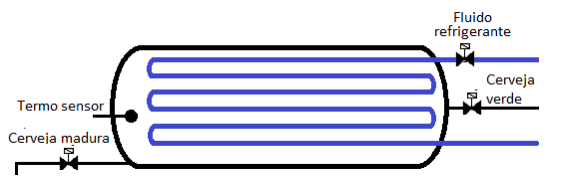
\includegraphics [width=0.5\linewidth]{tanque.png}
		\caption {Tanque de maturação da cerveja verde.}
		\label{fig:maturador}
	\end{figure}
\end{frame}
%------------------------------------------------
\subsection{Filtragem}
\begin{frame}
	\frametitle{Filtragem}
	\begin{itemize}
		\item Liberação da cerveja madura e da terra diatomácea
		\item Descarte dos resíduos
	\end{itemize}
	
	
	\begin{figure}[H]
		\centering
		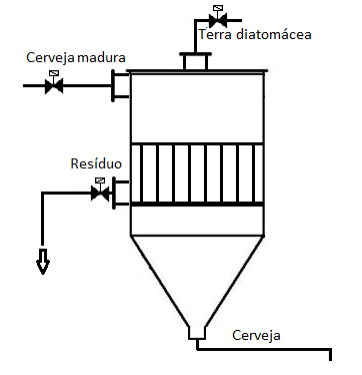
\includegraphics [width=0.3\linewidth]{filtro.png}
		\caption {Filtro da cerveja maturada}
		\label{fig:filtro}
	\end{figure}
\end{frame}

%------------------------------------------------
\section{Análise do Projeto}
\begin{frame}
\frametitle{Análise do Projeto}
	\begin{block}{Considerações}
		\begin{itemize}
		\item Sensor de nível baixo para maturador
		\item Tempo para enchimento: 10 minutos
		\item Filtragem e liberação de resíduos em paralelo com enchimento e maturação
		\item Sensor de nível abaixo do filtro.
		\end{itemize}
	\end{block}
\end{frame}

\begin{frame}
	\frametitle{Análise do Projeto}
	\begin{block}{Especificações}
		\begin{itemize}
			\item Monitoração de anomalias na operação
			\item Modo de emergência
			\item Modos de operação (Passo a passo e automático)
			\item Supervisor para monitoramento.
		\end{itemize}
	\end{block}
\end{frame}
%------------------------------------------------
\subsection{Tabela de Designação}
\begin{frame}
	\begin{block}{Tabela de Entradas}
	\begin{table}[H]
	\centering
	\begin{tabular}{|  p{0.15\linewidth} | p{0.55\linewidth} | }
		\hline
		Entrada & Utilidade\\
		\hline
		$S_{bm}$ & Sensor de volume baixo no tanque de maturação \\
		$S_t$ & Sensor de temperatura no tanque de maturação \\
		$S_{bf}$ & Sensor de volume baixo do filtro \\
		\hline
		\end{tabular}
	\end{table}
	\end{block}
\end{frame}
%------------------------------------------------
\begin{frame}
	\begin{block}{Tabela de Saídas}
		\begin{table}[H]
			\centering
			\begin{tabular}{|  p{0.15\linewidth} | p{0.55\linewidth} | }
				\hline
				Atuador & Utilidade\\
				\hline
				$V_{cv}$ & Acionamento da válvula da cerveja verde \\
				$V_{cm}$ & Acionamento da válvula da cerveja maturada \\
				$V_{fr}$ & Acionamento da válvula de fluido refrigerante \\
				$V_{td}$ & Acionamento da válvula de terra diatomácea \\
				$V_r$ & Acionamento da válvula de descarte \\
				\hline
			\end{tabular}
		\end{table}
	\end{block}
\end{frame}
%------------------------------------------------
\subsection{Supervisório}
\begin{frame}
	\frametitle{Supervisório}
		\begin{itemize}
			\item Mostrar anomalias
			\item Controle do modo de operação passo a passo
			\item Seleção do modo de operação
			\item Botão de emergência
			\item Acompanhamento da temperatura
		\end{itemize}
\end{frame}

%----------------------------------------------------------------------------------------

\end{document} 